\newpage
\section{Smooth Shading}
To compute the color of each pixel the \textbf{rendering equation} is used. Objects are made of \textbf{meshes} , several faces  but to solve the rendering equation different approaches can be used:
\begin{itemize}
\item \textbf{Per-face computation}
\item \textbf{Per-vertex computation}
\item \textbf{Per-pixel computation} 
\end{itemize}
The smaller the per-object computation the more computational expensive it is. For a Full-HD screen the per-pixel computation requires solving the rendering equation 2 million times but the final result is more visually appealing than the one of the other methods. To guarantee good real-time results rendering should be performed using modern software and hardware techniques (i.e. shading languages executed on GPUs).
With current technology there is no gain in using per-face or per-vertex and since per-vertex gets the better final result the \textbf{per-face} computation is \textbf{no longer used}. The per-vertex and per-pixel computations allow to obtain \textbf{smooth shadings}.\\
Polygonal surfaces can be encoded in many ways (already seen) and often result in \textbf{sharp edges}. These edges can be rendered as \textbf{continuous surfaces} using \textbf{smooth shading} algorithms , with the main 2 being: 
\begin{itemize}
\item Gouraud shading (\textbf{per-vertex})
\item Phong shading ( \textbf{per-pixel})
\end{itemize}
Both techniques require extending the \textbf{encoding} of the \textbf{vertex} ( 3 additional normal vector components) : $$ v = (x,y,z,n_x,n_y,n_z)$$
\begin{figure}[H]
  \centering
  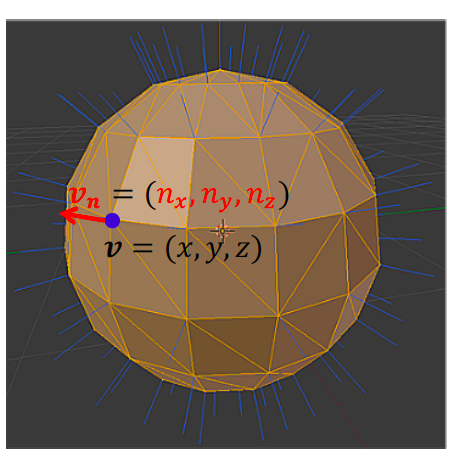
\includegraphics[width=.3\linewidth]{shading1}
\end{figure}
The normal is used to compute the color in the rendering equation.\\
As seen meshes are composed of \textbf{triangles} , which has three vertexes . Each triangle has a \textbf{normal} to its surface (identical in all points of the triangle).
\begin{figure}[H]
  \centering
  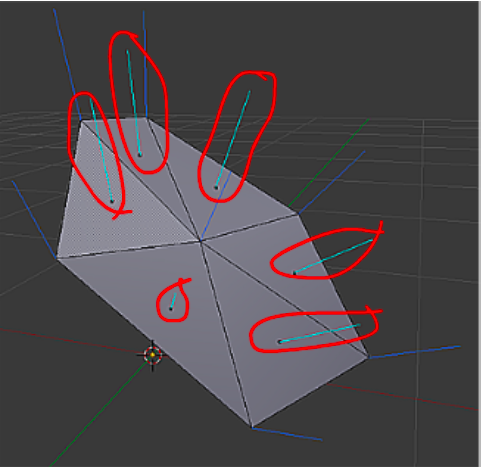
\includegraphics[width=.3\linewidth]{shading2}
\end{figure}
Adjacent surfaces can have very different normal vectors and this abrupt change can cause abrupt changes in the \textbf{color}. The result is the effect of a \textbf{not smooth} color transition.\\
With \textbf{shading techniques} this does not happen : they store for each vertex the Cartesian coordinates and the direction of the normal vector to the \textbf{original surface}. So instead of using for each pixel on the face the normal (equal for all points of the surface) the corresponding normal is computed via \textbf{interpolation} starting from the \textbf{3 vertexes} that make up the triangle.
\begin{figure}[H]
  \centering
  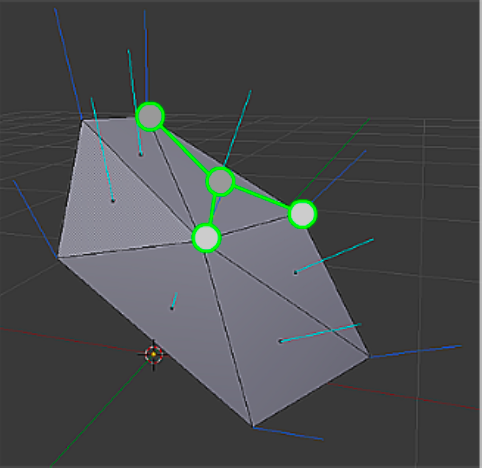
\includegraphics[width=.3\linewidth]{shading3}
\end{figure}
As already seen different vertexes can belong to different triangles. Depending on the triangle a vertex belongs to, its \textbf{normal vector changes}.
 \begin{figure}[H]
  \centering
  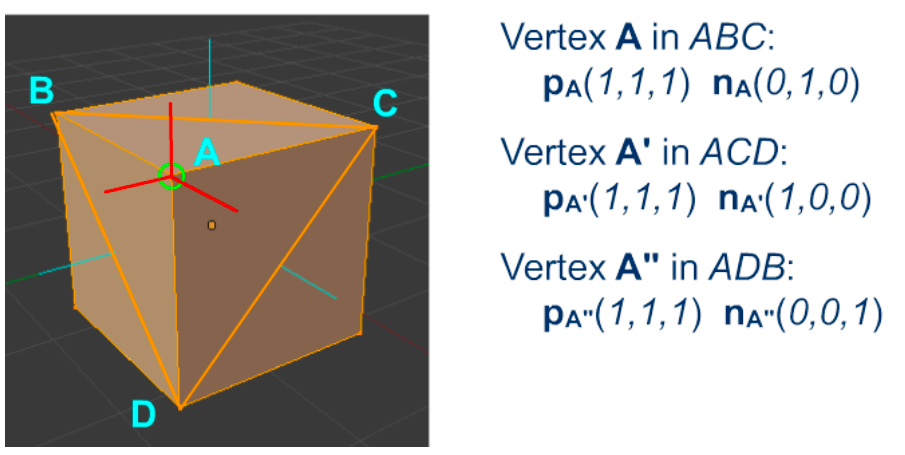
\includegraphics[width=.4\linewidth]{shadingnorm}
\end{figure}
If the norm for such shared vertexes is the \textbf{same} for all surfaces then the result is a \textbf{smooth surface}. So depending on the final effect , the normal vectors should be the \textbf{same} if a \textbf{smooth} effect is desired (like in a sphere) or should be \textbf{different}  if a \textbf{sharp-edge} effect is desired (like in a cube).
\subsection{Gouraud shading}
The Gouraud shading uses the \textbf{light} and \textbf{reflection } models to compute the color of each vertex. The colors of the \textbf{inner points} are computed using \textbf{interpolation }.\\
Vertex colors for static objects can be \textbf{pre-computed} and stored with the vertex geometry if:
\begin{itemize}
\item the objects is illuminated by \textbf{static lights}
\item the objects's material BRDF does not depend on the direction of the observer ( i.e. just \textbf{diffuse} component using the Lambert Model)
\end{itemize}

\subsection{Phong shading}
(Not be confused with Phong reflection model!)\\
This technique compute the color for \textbf{each pixel} separately. In this case \textbf{vertex normal vectors} are interpolated to \textbf{approximate}  the normal vector to the actual surface (the Gouraud techniques directly interpolates the color).This can lead to inner normal vectors the are \textbf{longer} the the unit. To avoid this at each step a \textbf{normalization} must be performed.\\
The last step is to compute the illumination model for every pixel using the \textbf{interpolated} normal vectors.\\
The \textbf{normalization} step together with solving the rendering equation for \textbf{each pixel} makes the Phong shading technique very expensive but nonetheless it achieves very good results. On the other hand the Gouraud is less complex but can sometimes result in \textbf{less appealing} visual effects because the techniques \textbf{misses} some important illumination / shading details. Generally speaking if the number of vertex is very high ( so each triangle is only a few pixels big) then the performances are \textbf{almost equivalent}.

\subsection{Transformations of normal vectors}
Since the normal vector are now stored with the objects the must behave correctly in the case of \textbf{view} and \textbf{world} \textbf{transformations} .Normal vectors however  don't follow the same computations: they are \textbf{3D directions}
composed of three components  and \textbf{not homogeneous coordinates} (with 4 components).The \textbf{transform} matrix for the \textbf{normal} vectors can be obtained starting from the 4x4 matrix that transforms homogeneous coordinates by computing the \textbf{inverse transpose} of its 3x3 \textbf{upper-left sub-matrix}:
 